\documentclass[journal]{IEEEtran}

\usepackage{cite}
\usepackage{amsmath,amssymb}
\usepackage{graphicx}
\usepackage{booktabs}
\usepackage{multirow}
\usepackage{url}
\usepackage[ruled,linesnumbered,vlined]{algorithm2e}

\graphicspath{{figures/}}
\newcommand{\Bel}{\mathrm{Bel}}
\newcommand{\BetP}{\mathrm{BetP}}
\SetKwInput{KwPar}{Parameters}
\SetKwInput{KwProc}{Procedure}

\markboth{IEEE TRANSACTIONS ON FUZZY SYSTEMS (MANUSCRIPT DRAFT)}%
{AUTHOR NAMES: EFFICIENT AND EVIDENCE-PRESERVING BFI CLUSTERING}

\begin{document}

\title{An Efficient and Evidence-Preserving Framework for Belief-Based Fuzzy and Imprecise Clustering}

\author{Author Name 1, Author Name 2, and Author Name 3%
\thanks{Author Name 1, Author Name 2, and Author Name 3 are with the Department of \ldots, \ldots\ University, City, Country (e-mail: \ldots).}%
\thanks{Replace these placeholders with the full names and affiliations of all team members.}%
}

\maketitle

\begin{abstract}
Belief-based fuzzy and imprecise clustering (BFI) detects clusters of arbitrary shapes through belief-based density peaks and evidential convergence, and assigns ambiguous objects to meta-clusters. However, its reference formulation computes and sorts the full $N\times N$ distance matrix, i.e., $O(N^2\log N)$ time and $O(N^2)$ memory, and its authors identify the long execution time as its main limitation. To address this issue, this article investigates an efficient and evidence-preserving BFI that changes only how neighbours are retrieved. First, an adaptive candidate neighbour retrieval gives every object a short, sorted, exact candidate list from a k-d tree. Sufficiency certificates prove when such a list answers the two search queries of BFI exactly, and only the lists that fail the certificate are enlarged. Second, an exact distance-based refinement computes the belief values from exact neighbour distances streamed in bounded memory and resolves the few uncertified queries by exact scans restricted to the relevant subset. With an exact distance factor, the proposed method reproduces the output of the original BFI exactly, including the meta-clusters (label agreement $1.000\pm0.000$ on 13 datasets $\times$ 5 seeds). Peak memory falls from 366\,MB to 26\,MB at $N=4000$, and 50\,000 objects are clustered with 38\,MB, where the distance matrix alone would need about 20\,GB. The method is up to $2.3\times$ faster at the largest size the original could run. The cases where the acceleration does not help are also reported.
\end{abstract}

\begin{IEEEkeywords}
Clustering, density peaks, evidence theory, imprecision, nearest-neighbour search, scalability.
\end{IEEEkeywords}

%======================================================================
\section{Introduction}
%======================================================================
\IEEEPARstart{R}{eal-world} datasets often contain complex structures characterized by irregular cluster shapes, varying densities, overlapping regions, and noisy observations. Such characteristics are commonly encountered in image segmentation, pattern recognition, medical image analysis, and other data-driven applications. For instance, in image segmentation, neighbouring pixels may exhibit similar features while pixels near object boundaries can share characteristics of multiple regions, making precise assignment difficult. Similarly, in multidimensional datasets, clusters may differ significantly in size and density, creating challenges for conventional clustering techniques. These characteristics make it important to develop clustering approaches that can identify complex data distributions while representing uncertainty and ambiguity in cluster membership.

To address these challenges, several unsupervised clustering approaches have been developed, including partition-based, fuzzy-based, and density-based techniques. Partition-based methods group observations according to their similarity to predefined cluster representatives, while fuzzy clustering assigns membership degrees to multiple clusters to represent gradual membership. Density-based approaches identify clusters through the distribution and concentration of neighbouring observations and can discover clusters with irregular shapes. More recently, evidential clustering methods have incorporated evidence theory to represent uncertainty and imprecision through belief assignments over individual clusters and combinations of clusters \cite{zhang2025survey}.

Among the existing approaches, K-means and fuzzy C-means are widely studied partition-based and fuzzy clustering methods, respectively \cite{macqueen1967, bezdek1981}. DBSCAN identifies dense regions and separates noise \cite{ester1996}, whereas Mean Shift detects clusters through density estimation \cite{comaniciu2002}. Density Peaks Clustering (DPC), introduced by Rodriguez and Laio, identifies potential cluster centres using local density and distance from higher-density observations \cite{rodriguez2014}. Several extensions have subsequently investigated improvements in scalability, centre detection, and data allocation \cite{du2016, xie2016, guan2024, yu2026}. Evidential clustering methods further incorporate belief functions to represent ambiguous membership \cite{masson2008, su2019}. In 2025, Zhang \emph{et al.} proposed Belief-Based Fuzzy and Imprecise Clustering (BFI), combining belief-based density-peak detection and evidential convergence to identify arbitrary-shaped clusters and represent imprecise observations through meta-clusters \cite{zhang2025}.

Despite these developments, computational efficiency remains an important consideration when applying density-based and evidential clustering methods to larger datasets. The original BFI framework requires neighbour information, distance calculations, and evidence-based assignment operations during its clustering process. Its authors acknowledge that the method requires a relatively long execution time, limiting its applicability in some cases, and identify acceleration as future work \cite{zhang2025}. Moreover, acceleration must be evaluated not only in terms of execution time but also in terms of its impact on belief assignments, meta-cluster identification, and overall clustering quality. Without loss of generality, the question addressed in this article is as follows.

\emph{How can BFI be accelerated without changing its belief assignments and meta-clusters?}

To this end, we propose an efficient and evidence-preserving extension of BFI based on adaptive neighbour search. The main contributions are summarized in the following three aspects.
\begin{enumerate}
\item We propose an \emph{adaptive candidate neighbour retrieval} for BFI. Every object receives a short exact candidate list, and \emph{sufficiency certificates} prove when this list answers the $\delta$ query and the evidential-convergence query exactly. Only lists that fail the certificate are enlarged, so the candidate size follows the local data structure.
\item We design an \emph{exact distance-based refinement}. It computes the belief values from exact neighbour distances streamed in bounded memory and resolves uncertified queries by exact scans restricted to the higher-belief or allocated subset. Together with the first contribution, it provably reproduces the belief assignments and meta-clusters of the original BFI without forming the distance matrix.
\item We evaluate the method against the original BFI on 13 synthetic and real datasets with 5 seeds and on scalability data with up to 50\,000 objects. The evaluation covers clustering quality, evidential metrics, runtime, memory and neighbour-search accuracy. It is complemented by a factorial ablation, a parameter-sensitivity study, a negative result and an explicit list of limitations.
\end{enumerate}

The rest of this article is organized as follows. Section~\ref{sec:prelim} offers a concise overview of evidence theory, BFI and related works. Section~\ref{sec:method} introduces the proposed method. Section~\ref{sec:exp} is dedicated to assessing its efficiency and evidence preservation. In Section~\ref{sec:disc}, we discuss the complexity and limitations. Finally, Section~\ref{sec:concl} concludes this article.

%======================================================================
\section{Preliminaries}\label{sec:prelim}
%======================================================================
In this section, we provide a brief overview of evidence theory, of the BFI method, and of related works on evidential clustering and efficient density-peaks clustering.

\subsection{Basics of Evidence Theory}
Evidence theory \cite{dempster1967, shafer1976} extends the frame $\Omega=\{\omega_1,\dots,\omega_c\}$ to the power set $2^\Omega$. A basic belief assignment (BBA) $m:2^\Omega\to[0,1]$ satisfies
\begin{equation}
\sum_{A\in 2^{\Omega}} m(A)=1. \label{eq:bba_norm}
\end{equation}
A subset $A$ with $m(A)>0$ is a focal set. In clustering, $\{\omega_k\}$ is a singleton (precise) cluster, a subset with several clusters is a meta-cluster expressing imprecision, and $\emptyset$ is the noise cluster. Two BBAs are combined by Dempster's rule
\begin{equation}
[m_1\oplus m_2](A)=\frac{\sum_{B\cap C=A} m_1(B)\,m_2(C)}{1-\sum_{B\cap C=\emptyset} m_1(B)\,m_2(C)}. \label{eq:ds}
\end{equation}
A crisp decision is taken from the pignistic probability \cite{smets1990}
\begin{equation}
\BetP(\omega_k)=\sum_{A\ni\omega_k}\frac{m(A)}{|A|}. \label{eq:betp}
\end{equation}

\subsection{Belief-Based Fuzzy and Imprecise Clustering}
Consider a dataset $X=\{x_1,\dots,x_N\}$ with $d_{ij}=\|x_i-x_j\|$, and let $d_{i,(k)}$ be the $k$-th smallest distance from $x_i$ to another object. BFI \cite{zhang2025} consists of two steps.

\emph{1) Belief-based density peaks:} Each of the $K_1$ nearest neighbours $x_k$ of $x_i$ provides a mass function on $\Omega_C=\{C,U\}$ (centre / unknown) with $m_{ik}(C)=\tfrac{1}{K_1}e^{-\vartheta_i d_{ik}}$, where the distance factor is
\begin{equation}
\vartheta_i = 1/\mathrm{quantile}\big(\{d_{ij}: j\neq i\},\,q\big),\qquad q=0.9. \label{eq:theta}
\end{equation}
Combining the $K_1$ mass functions by (\ref{eq:ds}) gives the belief that $x_i$ is a centre:
\begin{equation}
\Bel_i(C)=1-\prod_{k=1}^{K_1}\Big(1-\frac{1}{K_1}e^{-\vartheta_i d_{i,(k)}}\Big). \label{eq:bel}
\end{equation}
The distance to the nearest object of higher belief is
\begin{equation}
\delta_i=\begin{cases}\max_j d_{ij}, & \text{if } \Bel_i\ge\Bel_j\ \forall j,\\ \min_{j:\Bel_i<\Bel_j} d_{ij}, & \text{otherwise,}\end{cases} \label{eq:delta}
\end{equation}
and the $c$ objects with the largest $\gamma_i$ in the decision graph are selected as cluster centres.

\emph{2) Evidential convergence:} The remaining objects are allocated in decreasing order of $\Bel$. For object $x_t$, the $K_2$ nearest \emph{already-allocated} objects $\mathcal{N}_t$ each provide $m^k_t(\{\omega_\varphi\})=e^{-\vartheta_t d_{tk}}$ for their cluster $\omega_\varphi$. The pieces of evidence supporting the same cluster are fused by (\ref{eq:ds}), which gives
\begin{equation}
m^{\varphi}_t=1-\prod_{x_k\in\mathcal{N}_t,\ \ell_k=\varphi}\big(1-e^{-\vartheta_t d_{tk}}\big). \label{eq:support}
\end{equation}
The clusters close to the strongest one form the adaptive frame
\begin{equation}
\mathcal{M}_t=\{\omega_\varphi : \max_{\psi} m^{\psi}_t - m^{\varphi}_t\le\zeta\}, \label{eq:mt}
\end{equation}
and every $A\subseteq\mathcal{M}_t$ receives the mass
\begin{equation}
m^{\mathcal{M}_t}(A)=\prod_{\omega_\varphi\in A} m^{\varphi}_t\prod_{\omega_\varphi\in\mathcal{M}_t\setminus A}\big(1-m^{\varphi}_t\big), \label{eq:bba}
\end{equation}
where $A=\emptyset$ gives the noise mass. The object is assigned to the focal set with the highest normalized BBA, or to the cluster with the highest $\BetP$ (\ref{eq:betp}) when a crisp decision is required.

\emph{Cost:} The reference implementation computes and sorts the full distance matrix, i.e., $O(N^2\log N)$ time and $O(N^2)$ memory, about 20\,GB at $N=50\,000$. Only three \emph{neighbour queries} need this matrix: the $K_1$ nearest distances for (\ref{eq:bel}), the nearest higher-belief object for (\ref{eq:delta}), and the $K_2$ nearest allocated objects for (\ref{eq:support}). The quantile (\ref{eq:theta}) needs all distances but not their storage.

\subsection{Related Works}
\emph{1) Evidential clustering:} ECM \cite{masson2008} is the evidential version of fuzzy C-means. EVCLUS \cite{denoeux2004} derives credal partitions from proximity data, credal C-means \cite{liu2015} models imprecision between clusters, and BPEC \cite{su2019} introduces belief peaks. These methods are partition-based, whereas BFI uses a density-peak strategy and therefore handles arbitrary shapes \cite{zhang2025}. A recent survey of evidential clustering is given in \cite{zhang2025survey}.

\emph{2) Efficient density-peaks clustering:} The quadratic cost of DPC \cite{rodriguez2014} has motivated kNN-based formulations \cite{du2016, xie2016}, computation restricted to relevant regions \cite{guan2024}, minimum-spanning-tree-based acceleration \cite{qiu2023}, and parallel clustering with graph-based approximate nearest-neighbour search \cite{yu2026}. Most of these methods change the density definition or the allocation rule, or accept approximate neighbours.

\emph{3) Nearest-neighbour search:} Exact $k$-NN queries in low dimension are answered by k-d trees \cite{bentley1975, friedman1977}, whose efficiency degrades in high dimension \cite{weber1998}. Approximate methods such as NN-Descent \cite{dong2011} and HNSW \cite{malkov2020} trade exactness for speed.

For BFI, every change of the neighbours changes the evidence: the belief values, $\delta$, the centres and every BBA. To our knowledge, no accelerated version of BFI has been published. Unlike the methods above, the proposed method keeps every formula of BFI and guarantees identical evidential output. We do not claim novelty for k-d-tree search or for computing exact Euclidean distances, both of which are standard.

%======================================================================
\section{Proposed Method}\label{sec:method}
%======================================================================
The proposed method is based on two observations. First, the three neighbour queries of BFI are \emph{local}: for most objects the answer lies among a few nearest neighbours, so a short candidate list usually suffices. Second, it can be \emph{proven} from a sorted exact list whether the list suffices, so exact computation is needed only for the few remaining queries. Based on these observations, the method consists of two components, presented in Sections~\ref{sec:s1} and \ref{sec:s2}. All evidential formulas (\ref{eq:theta})--(\ref{eq:bba}) are evaluated by the same code as in the original BFI.

\subsection{Solution 1: Adaptive Candidate Neighbour Retrieval}\label{sec:s1}
A k-d tree is built once in $O(N\log N)$. Every object $x_i$ receives a \emph{base list} $L_i$: its $k_{\min}=16$ nearest neighbours with exact distances, sorted by distance.

\emph{1) Sufficiency certificates:} Let $L_i^{(k)}$ be the exact $k$ nearest neighbours of $x_i$ in increasing order of distance.
\begin{enumerate}
\item[a)] \emph{$\delta$-certificate:} If $L_i^{(k)}$ contains an object with $\Bel_j>\Bel_i$, the first such object is the nearest higher-belief object overall, because every object closer to $x_i$ belongs to $L_i^{(k)}$ and has been checked.
\item[b)] \emph{Convergence certificate:} If, when $x_t$ is processed, $L_t^{(k)}$ contains at least $K_2$ allocated objects, its first $K_2$ allocated entries are exactly $\mathcal{N}_t$, for the same reason.
\end{enumerate}
A query answered under a certificate is therefore identical to the original's answer; it is not an approximation.

\emph{2) Adaptive growth:} A list that fails its certificate is regrown through the index to $2k, 4k, \ldots$ up to a budget $k_{\max}=512$. The candidate size thus adapts to the local data structure. Cluster cores are resolved by the base list, while density peaks, cluster borders, sparse regions and objects allocated early in the convergence, when few objects are allocated, search further. Queries still uncertified at $k_{\max}$ are passed to Solution~2. The procedure is summarized in Algorithm~\ref{alg:s1}.

\begin{algorithm}[!t]
\caption{Adaptive Candidate Neighbour Retrieval.}\label{alg:s1}
\KwIn{Data $X=\{x_1,\dots,x_N\}$; belief ranks; base lists $L_i$.}
\KwPar{$k_{\min}$, $k_{\max}$, $K_2$.}
\KwProc{}
\For{$i$ in $1:N$}{
  $k\gets k_{\min}$\;
  \While{$L_i^{(k)}$ has no object with higher $\Bel$ \textbf{and} $k<k_{\max}$}{
    $k\gets 2k$; obtain $L_i^{(k)}$ from the k-d tree\;
  }
  \lIf{certified}{$\delta_i\gets$ distance to first higher-$\Bel$ entry}
  \lElse{mark $x_i$ for exact refinement (Algorithm~\ref{alg:s2})}
}
Select the $c$ centres by $\gamma_i$\;
\For{$x_t$ in decreasing order of $\Bel$}{
  Grow $L_t^{(k)}$ in the same way until it holds $K_2$ allocated objects\;
  \lIf{certified}{$\mathcal{N}_t\gets$ first $K_2$ allocated entries}
  \lElse{mark $x_t$ for exact refinement (Algorithm~\ref{alg:s2})}
  Fuse evidence by (\ref{eq:support})--(\ref{eq:bba}) and allocate $x_t$\;
}
\KwRet{BBAs, $\BetP$, clustering results.}
\end{algorithm}

\subsection{Solution 2: Exact Distance-Based Refinement}\label{sec:s2}
\emph{1) Exact belief, streamed:} The exact $K_1$ nearest distances are obtained from the index for chunks of objects (at most $2^{19}$ entries per chunk). They are reduced immediately to the log-product of (\ref{eq:bel}) and then discarded. The first $k_{\min}$ columns are kept as the base lists of Solution~1. The memory is $O(Nk_{\min}+\text{chunk})$ instead of $O(N^2)$.

\emph{2) Restricted exact scans:} A $\delta$ query not certified within $k_{\max}$ is answered by computing distances only to the $\mathrm{rank}(i)$ objects with higher belief. An uncertified convergence query is answered by computing distances only to the currently allocated objects.

\emph{3) Exact distance factor:} Eq.~(\ref{eq:theta}) is computed by chunked distance blocks and partial selection, without sorting and in $O(N)$ memory. Optionally, $\vartheta$ is estimated from a random reference sample of $s=1000$ objects, which reduces this step from $O(N^2)$ to $O(Ns)$ time. This is the \emph{only} approximation in the practical configuration. The procedure is summarized in Algorithm~\ref{alg:s2}.

\begin{algorithm}[!t]
\caption{Exact Distance-Based Refinement.}\label{alg:s2}
\KwIn{Data $X$; $K_1$; queries marked by Algorithm~\ref{alg:s1}.}
\KwPar{chunk budget, $q$, optional sample size $s$.}
\KwProc{}
Compute $\vartheta_i$ by (\ref{eq:theta}) with chunked partial selection (or from $s$ samples)\;
\For{each chunk $R$ of objects}{
  Obtain the exact $K_1$ nearest distances of $R$ from the k-d tree\;
  Compute $\Bel_i$ by (\ref{eq:bel}); keep the first $k_{\min}$ neighbours as $L_i$\;
}
\For{each marked $\delta$ query $x_i$}{
  $\delta_i\gets\min_{j:\Bel_j>\Bel_i} d_{ij}$ over the higher-belief subset only\;
}
\For{each marked convergence query $x_t$}{
  $\mathcal{N}_t\gets$ $K_2$ nearest objects among the allocated subset only\;
}
\KwRet{$\vartheta$, $\Bel$, exact $\delta$ and $\mathcal{N}_t$.}
\end{algorithm}

\subsection{Exactness of the Proposed Method}
\emph{Proposition:} With exact $\vartheta$, the proposed method (Solution~1 + Solution~2) returns the same $\Bel$, $\delta$, centres, BBAs, pignistic probabilities and meta-clusters as the original BFI, up to floating-point rounding, for any $k_{\min}\le k_{\max}$.

\emph{Reason:} $\Bel$ uses the exact $K_1$ nearest distances. Every $\delta$ and convergence query is answered either under a certificate or by an exact scan of the complete candidate subset. The evidential formulas are shared with the original. This was verified by unit tests for several $(k_{\min},k_{\max})$, including the degenerate $k_{\max}=3$.

\subsection{Parameters Involved}
The proposed method keeps the BFI parameters $K_1$, $K_2$, $\zeta$ and $q$. It adds:
\begin{enumerate}
\item $k_{\min}$, the initial list size;
\item $k_{\max}$, the growth budget;
\item optionally $s$, the $\vartheta$ sample size.
\end{enumerate}
With exact $\vartheta$, $k_{\min}$ and $k_{\max}$ affect only the speed and never the result. They were set by the ablation in Experiment~3 to $k_{\min}=16$ and $k_{\max}=512$. Two deviations from the literal BFI are applied identically to the original and to all variants:
\begin{enumerate}
\item centres are selected by $\gamma_i=\Bel_i\,\delta_i$ instead of $\rho_{f(i)}\delta_i$ with $\rho_{f(i)}=e^{\delta_i}$, because the latter is monotone in $\delta_i$ and selected isolated outliers in our tests;
\item $K_2=3$, because with literal Dempster fusion $K_2=9$ lets several far neighbours outweigh a near one (confirmed in Experiment~4).
\end{enumerate}

%======================================================================
\section{Experiment Applications}\label{sec:exp}
%======================================================================
This part is dedicated to assessing the efficiency and the evidence preservation of the proposed method in comparison to the original BFI across various benchmark datasets.

\subsection{Benchmark Datasets}
We use synthetic, high-dimensional and real-world datasets, all min-max scaled, as follows.
\begin{enumerate}
\item Six 2-D synthetic datasets with $N=3000$ generated with scikit-learn \cite{pedregosa2011}:
\begin{itemize}
\item \emph{moons}, \emph{circles} and \emph{anisotropic}: non-convex and elongated shapes;
\item \emph{blobs\_separated} and \emph{blobs\_overlap}: separated and overlapping clusters;
\item \emph{varied\_density}: three clusters with standard deviations 1.0, 2.5 and 0.5.
\end{itemize}
A seed changes the sampled points but not the cluster layout.
\item Two high-dimensional synthetic datasets, \emph{blobs\_hd8} and \emph{blobs\_hd32}, with $N=3000$, $d=8$ and $d=32$, and five overlapping clusters.
\item Five real-world datasets: \emph{iris} ($N=150$, $d=4$), \emph{wine} (178, 13), \emph{breast\_cancer} (569, 30), and handwritten \emph{digits} with 6 classes reduced by PCA to 10 dimensions (1083, 10) or 10 classes reduced to 16 dimensions (1797, 16).
\item A scalability dataset: a four-component 2-D Gaussian mixture with $N$ from 1000 to 50\,000.
\end{enumerate}
Unless stated otherwise, $K_1=\max(10,0.06N)$, $K_2=3$, $\zeta=0.1$ and $q=0.9$.

\subsection{Evaluation Criteria}
Following \cite{zhang2025}, we use the following criteria.
\begin{itemize}
\item \emph{Clustering}: the error rate ($R_e$), the imprecision rate ($R_i$), Precision ($P$), Recall ($R$) and Rand Index ($RI$) of the crisp result, together with their evidential versions EP, ER and ERI \cite{zhang2025survey, liu2015}. We use a simplified pairwise-credal variant of EP, ER and ERI.
\item \emph{Agreement-adjusted}: ARI \cite{hubert1985}, AMI and NMI \cite{strehl2002}.
\item \emph{Evidence preservation}, measured against the original BFI on the same data:
\begin{itemize}
\item label agreement after Hungarian alignment \cite{kuhn1955};
\item the mean total-variation distance between the pignistic probabilities (BetP TV);
\item focal-set agreement, i.e., identical singleton or meta-cluster assignment.
\end{itemize}
\item \emph{Efficiency}: wall time (median of 3 runs), the additional peak memory of one run in a fresh process, and the speed-up $t_{\mathrm{orig}}/t$.
\item \emph{Neighbour search}: candidate recall and final selection accuracy of the $\delta$ and convergence neighbours.
\end{itemize}
Except for $R_e$ and $R_i$, a higher value indicates a better result.

\subsection{Comparison Methods}
Five configurations are compared in a $2\times2$ factorial design around the reference:
\begin{enumerate}
\item \emph{Original BFI}: the full distance matrix;
\item \emph{Control}: fixed 64-nearest-neighbour lists, without adaptivity or refinement, i.e., a naive kNN-BFI;
\item \emph{S1}: adaptive retrieval only, with uncertified queries estimated;
\item \emph{S2}: fixed lists with exact refinement;
\item \emph{S1+S2}: the proposed method.
\end{enumerate}
The accelerated variants are run with exact $\vartheta$, which isolates the neighbour search, and with $\vartheta$ sampled from $s=1000$ objects (S1+S2$^{\dagger}$), the practical setting. Five seeds are used in Experiment~1 and three in Experiments~2--5; results are reported as mean $\pm$ standard deviation, without formal significance tests. All methods run single-threaded on a 16-core Windows~11 laptop with 15.7\,GB RAM (Python~3.11, NumPy \cite{harris2020}, SciPy \cite{virtanen2020}, scikit-learn \cite{pedregosa2011}).

\subsection{Results and Analysis}
Within this part, we present and examine the results. Experiment~1 evaluates clustering quality and evidence preservation on the 13 datasets. Experiment~2 investigates scalability. Experiment~3 analyses the contribution of each component. Experiment~4 studies parameter sensitivity, and Experiment~5 reports a negative result.

\emph{1) Experiment 1:} Tables~\ref{tab:synthetic} and \ref{tab:real} display the outcomes of the methods on the synthetic and real-world datasets. Table~\ref{tab:agree} summarizes the agreement with the original BFI, and Fig.~\ref{fig:clusters} shows the clustering results on the six 2-D datasets. The following observations can be made.
\begin{enumerate}
\item[a)] With exact $\vartheta$, S2 and S1+S2 reproduce the original BFI on every dataset and seed. All eleven criteria in Tables~\ref{tab:synthetic} and \ref{tab:real} are identical, the label agreement is $1.000\pm0.000$, the BetP distance is $0$, and the focal sets, including all meta-cluster assignments, coincide (Table~\ref{tab:agree}). The evidential output of BFI is therefore fully preserved.
\item[b)] Without refinement, the clustering changes. On \emph{moons}, ARI drops from 0.998 to 0.530 for the control and to 0.822 for S1. On iris, wine and the high-dimensional blobs, the control instead \emph{raises} ARI (e.g., wine $0.443\rightarrow0.835$). However, it agrees with the original on only 83.3\% of the objects on average, so this is a different clustering produced by approximation, not a preserved BFI result.
\item[c)] With sampled $\vartheta$ (S1+S2$^{\dagger}$), the ARI stays within $\pm0.003$ of the original on the six 2-D datasets. They decrease on the four high-dimensional datasets (e.g., digits6 ARI $0.546\rightarrow0.413$), where BFI's sequential convergence amplifies small perturbations of $\vartheta$.
\item[d)] \emph{circles} and \emph{breast\_cancer} have ARI $\approx0$ for every method, including the original. This is a limitation of the density-peak centre selection, not of the acceleration.
\end{enumerate}

Table~\ref{tab:efficiency} reports the runtime per dataset. On the 2-D datasets, S1+S2$^{\dagger}$ is $1.98$--$2.29\times$ faster than the original ($1.44$--$1.67\times$ with exact $\vartheta$), and peak memory falls from 206\,MB to 18--19\,MB. On blobs\_hd32 and on the small real datasets there is no speed-up (Section~\ref{sec:disc}).

The short initial lists of 16 entries already contain 99.2\% of the true $\delta$-neighbours and 98.2\% of the true convergence neighbours. Growth and refinement handle the rest, so the final selection accuracy of S1+S2 is 1.000 (Fig.~\ref{fig:neigh}).

\begin{table*}[!t]
\centering
\caption{Clustering results of the original BFI and the accelerated variants on the eight synthetic datasets}
\label{tab:synthetic}
\scriptsize
\setlength{\tabcolsep}{4.2pt}
\begin{tabular}{llccccccccccc}
\toprule
Datasets & Methods & $R_e$ & $R_i$ & $P$ & $R$ & $RI$ & $EP$ & $ER$ & $ERI$ & ARI & AMI & NMI \\
\midrule
\multirow{6}{*}{moons} & Original BFI & \textbf{0.0002} & 0.0003 & \textbf{0.9992} & \textbf{0.9992} & \textbf{0.9992} & \textbf{0.9996} & \textbf{0.9996} & \textbf{0.9996} & \textbf{0.9984} & \textbf{0.9960} & \textbf{0.9960} \\
 & Control & 0.1342 & 0.0073 & 0.7650 & 0.7656 & 0.7652 & 0.7760 & 0.7789 & 0.7771 & 0.5305 & 0.4304 & 0.4305 \\
 & S1 & 0.0457 & 0.0037 & 0.9066 & 0.9171 & 0.9111 & 0.9182 & 0.9238 & 0.9206 & 0.8222 & 0.7854 & 0.7854 \\
 & S2 & \textbf{0.0002} & 0.0003 & \textbf{0.9992} & \textbf{0.9992} & \textbf{0.9992} & \textbf{0.9996} & \textbf{0.9996} & \textbf{0.9996} & \textbf{0.9984} & \textbf{0.9960} & \textbf{0.9960} \\
 & S1+S2 & \textbf{0.0002} & 0.0003 & \textbf{0.9992} & \textbf{0.9992} & \textbf{0.9992} & \textbf{0.9996} & \textbf{0.9996} & \textbf{0.9996} & \textbf{0.9984} & \textbf{0.9960} & \textbf{0.9960} \\
 & S1+S2$^{\dagger}$ & \textbf{0.0002} & 0.0003 & \textbf{0.9992} & \textbf{0.9992} & \textbf{0.9992} & \textbf{0.9996} & \textbf{0.9996} & \textbf{0.9996} & \textbf{0.9984} & \textbf{0.9960} & \textbf{0.9960} \\
\midrule
\multirow{6}{*}{circles} & Original BFI & 0.4733 & 0.0137 & 0.5009 & 0.5362 & 0.5011 & 0.5004 & 0.5388 & 0.5008 & 0.0022 & 0.0018 & 0.0020 \\
 & Control & 0.4677 & 0.0157 & \textbf{0.5015} & 0.5026 & \textbf{0.5017} & 0.5011 & 0.5012 & 0.5013 & \textbf{0.0034} & \textbf{0.0024} & \textbf{0.0027} \\
 & S1 & \textbf{0.4645} & 0.0185 & 0.5010 & \textbf{0.5517} & 0.5012 & \textbf{0.5013} & \textbf{0.5458} & \textbf{0.5017} & 0.0025 & 0.0023 & 0.0026 \\
 & S2 & 0.4733 & 0.0137 & 0.5009 & 0.5362 & 0.5011 & 0.5004 & 0.5388 & 0.5008 & 0.0022 & 0.0018 & 0.0020 \\
 & S1+S2 & 0.4733 & 0.0137 & 0.5009 & 0.5362 & 0.5011 & 0.5004 & 0.5388 & 0.5008 & 0.0022 & 0.0018 & 0.0020 \\
 & S1+S2$^{\dagger}$ & 0.4724 & 0.0144 & 0.5009 & 0.5387 & 0.5011 & 0.5003 & 0.5439 & 0.5006 & 0.0022 & 0.0018 & 0.0020 \\
\midrule
\multirow{6}{*}{aniso.} & Original BFI & \textbf{0.0029} & 0.0027 & \textbf{0.9928} & \textbf{0.9928} & \textbf{0.9952} & \textbf{0.9914} & \textbf{0.9915} & \textbf{0.9943} & \textbf{0.9893} & \textbf{0.9798} & \textbf{0.9798} \\
 & Control & 0.1978 & 0.0072 & 0.7565 & 0.9238 & 0.8558 & 0.7465 & 0.9263 & 0.8478 & 0.7092 & 0.7921 & 0.7923 \\
 & S1 & 0.0033 & 0.0025 & 0.9924 & 0.9925 & 0.9950 & \textbf{0.9914} & \textbf{0.9915} & \textbf{0.9943} & 0.9887 & 0.9788 & 0.9788 \\
 & S2 & \textbf{0.0029} & 0.0027 & \textbf{0.9928} & \textbf{0.9928} & \textbf{0.9952} & \textbf{0.9914} & \textbf{0.9915} & \textbf{0.9943} & \textbf{0.9893} & \textbf{0.9798} & \textbf{0.9798} \\
 & S1+S2 & \textbf{0.0029} & 0.0027 & \textbf{0.9928} & \textbf{0.9928} & \textbf{0.9952} & \textbf{0.9914} & \textbf{0.9915} & \textbf{0.9943} & \textbf{0.9893} & \textbf{0.9798} & \textbf{0.9798} \\
 & S1+S2$^{\dagger}$ & 0.0031 & 0.0029 & 0.9922 & 0.9922 & 0.9948 & 0.9908 & 0.9908 & 0.9939 & 0.9883 & 0.9782 & 0.9782 \\
\midrule
\multirow{6}{*}{blobs\_sep.} & Original BFI & \textbf{0.0040} & 0.0039 & \textbf{0.9891} & \textbf{0.9891} & \textbf{0.9928} & \textbf{0.9875} & \textbf{0.9871} & \textbf{0.9916} & \textbf{0.9837} & \textbf{0.9695} & \textbf{0.9696} \\
 & Control & 0.1749 & 0.0099 & 0.8184 & 0.9372 & 0.8878 & 0.8154 & 0.9461 & 0.8851 & 0.7758 & 0.8426 & 0.8427 \\
 & S1 & 0.0041 & 0.0045 & 0.9887 & 0.9888 & 0.9925 & 0.9853 & 0.9848 & 0.9900 & 0.9831 & 0.9690 & 0.9690 \\
 & S2 & \textbf{0.0040} & 0.0039 & \textbf{0.9891} & \textbf{0.9891} & \textbf{0.9928} & \textbf{0.9875} & \textbf{0.9871} & \textbf{0.9916} & \textbf{0.9837} & \textbf{0.9695} & \textbf{0.9696} \\
 & S1+S2 & \textbf{0.0040} & 0.0039 & \textbf{0.9891} & \textbf{0.9891} & \textbf{0.9928} & \textbf{0.9875} & \textbf{0.9871} & \textbf{0.9916} & \textbf{0.9837} & \textbf{0.9695} & \textbf{0.9696} \\
 & S1+S2$^{\dagger}$ & 0.0041 & 0.0038 & 0.9890 & 0.9890 & 0.9927 & \textbf{0.9875} & \textbf{0.9871} & 0.9915 & 0.9835 & 0.9693 & 0.9693 \\
\midrule
\multirow{6}{*}{blobs\_ovl.} & Original BFI & 0.1284 & 0.0236 & 0.7511 & 0.7549 & 0.8350 & 0.7426 & 0.7445 & 0.8287 & 0.6291 & 0.5623 & 0.5626 \\
 & Control & 0.2919 & 0.0307 & 0.6106 & 0.7257 & 0.7443 & 0.6038 & 0.7287 & 0.7373 & 0.4595 & 0.4748 & 0.4751 \\
 & S1 & \textbf{0.1259} & 0.0331 & 0.7483 & 0.7511 & 0.8329 & 0.7439 & 0.7450 & 0.8294 & 0.6243 & 0.5573 & 0.5576 \\
 & S2 & 0.1284 & 0.0236 & 0.7511 & 0.7549 & 0.8350 & 0.7426 & 0.7445 & 0.8287 & 0.6291 & 0.5623 & 0.5626 \\
 & S1+S2 & 0.1284 & 0.0236 & 0.7511 & 0.7549 & 0.8350 & 0.7426 & 0.7445 & 0.8287 & 0.6291 & 0.5623 & 0.5626 \\
 & S1+S2$^{\dagger}$ & 0.1261 & 0.0245 & \textbf{0.7533} & \textbf{0.7565} & \textbf{0.8364} & \textbf{0.7450} & \textbf{0.7469} & \textbf{0.8303} & \textbf{0.6321} & \textbf{0.5638} & \textbf{0.5641} \\
\midrule
\multirow{6}{*}{varied} & Original BFI & 0.0435 & 0.0105 & 0.9060 & 0.9154 & 0.9402 & 0.8960 & 0.9101 & 0.9347 & 0.8657 & 0.8442 & 0.8443 \\
 & Control & 0.2018 & 0.0123 & 0.7069 & 0.8713 & 0.8195 & 0.7145 & 0.8719 & 0.8242 & 0.6309 & 0.6681 & 0.6684 \\
 & S1 & \textbf{0.0407} & 0.0104 & \textbf{0.9104} & \textbf{0.9189} & \textbf{0.9429} & \textbf{0.9045} & \textbf{0.9167} & \textbf{0.9399} & \textbf{0.8717} & \textbf{0.8491} & \textbf{0.8491} \\
 & S2 & 0.0435 & 0.0105 & 0.9060 & 0.9154 & 0.9402 & 0.8960 & 0.9101 & 0.9347 & 0.8657 & 0.8442 & 0.8443 \\
 & S1+S2 & 0.0435 & 0.0105 & 0.9060 & 0.9154 & 0.9402 & 0.8960 & 0.9101 & 0.9347 & 0.8657 & 0.8442 & 0.8443 \\
 & S1+S2$^{\dagger}$ & 0.0435 & 0.0108 & 0.9056 & 0.9151 & 0.9399 & 0.8955 & 0.9096 & 0.9344 & 0.8651 & 0.8437 & 0.8438 \\
\midrule
\multirow{6}{*}{hd8} & Original BFI & 0.2982 & 0.0021 & 0.6038 & 0.9284 & 0.8598 & 0.5966 & \textbf{0.9286} & 0.8572 & 0.6415 & 0.7424 & 0.7429 \\
 & Control & \textbf{0.2044} & 0.0053 & \textbf{0.6812} & 0.9036 & \textbf{0.8945} & \textbf{0.6786} & 0.9019 & \textbf{0.8931} & \textbf{0.7077} & 0.7779 & 0.7783 \\
 & S1 & 0.2241 & 0.0023 & 0.6600 & 0.9246 & 0.8898 & 0.6556 & 0.9226 & 0.8875 & 0.7003 & \textbf{0.7818} & \textbf{0.7822} \\
 & S2 & 0.2982 & 0.0021 & 0.6038 & 0.9284 & 0.8598 & 0.5966 & \textbf{0.9286} & 0.8572 & 0.6415 & 0.7424 & 0.7429 \\
 & S1+S2 & 0.2982 & 0.0021 & 0.6038 & 0.9284 & 0.8598 & 0.5966 & \textbf{0.9286} & 0.8572 & 0.6415 & 0.7424 & 0.7429 \\
 & S1+S2$^{\dagger}$ & 0.3389 & 0.0018 & 0.5526 & \textbf{0.9288} & 0.8252 & 0.5440 & 0.9250 & 0.8210 & 0.5810 & 0.7074 & 0.7079 \\
\midrule
\multirow{6}{*}{hd32} & Original BFI & 0.2613 & 0.0048 & 0.6217 & 0.9473 & 0.8506 & 0.6289 & 0.9449 & 0.8564 & 0.6452 & 0.7732 & 0.7736 \\
 & Control & 0.1328 & 0.0077 & 0.7841 & 0.9304 & 0.9293 & 0.7905 & 0.9390 & 0.9323 & 0.8011 & 0.8422 & 0.8425 \\
 & S1 & \textbf{0.0820} & 0.0098 & \textbf{0.8521} & 0.9205 & \textbf{0.9487} & \textbf{0.8576} & 0.9239 & \textbf{0.9512} & \textbf{0.8491} & \textbf{0.8585} & \textbf{0.8587} \\
 & S2 & 0.2613 & 0.0048 & 0.6217 & 0.9473 & 0.8506 & 0.6289 & 0.9449 & 0.8564 & 0.6452 & 0.7732 & 0.7736 \\
 & S1+S2 & 0.2613 & 0.0048 & 0.6217 & 0.9473 & 0.8506 & 0.6289 & 0.9449 & 0.8564 & 0.6452 & 0.7732 & 0.7736 \\
 & S1+S2$^{\dagger}$ & 0.3038 & 0.0037 & 0.5680 & \textbf{0.9515} & 0.8193 & 0.5702 & \textbf{0.9487} & 0.8242 & 0.5871 & 0.7486 & 0.7491 \\
\bottomrule
\end{tabular}
\vspace{2pt}
\parbox{\textwidth}{\footnotesize Mean over seeds (5 for synthetic data; real data are deterministic). All variants with exact $\theta$ except S1+S2$^{\dagger}$ ($\theta$ sampled from 1000 objects). Bold: best value per dataset (lowest for $R_e$); $R_i$ is not ranked.}
\end{table*}

\begin{table*}[!t]
\centering
\caption{Clustering results of the original BFI and the accelerated variants on the five real-world datasets}
\label{tab:real}
\scriptsize
\setlength{\tabcolsep}{4.2pt}
\begin{tabular}{llccccccccccc}
\toprule
Datasets & Methods & $R_e$ & $R_i$ & $P$ & $R$ & $RI$ & $EP$ & $ER$ & $ERI$ & ARI & AMI & NMI \\
\midrule
\multirow{6}{*}{iris} & Original BFI & 0.1200 & 0.0200 & 0.7694 & 0.8299 & 0.8623 & 0.7671 & 0.8243 & 0.8599 & 0.6941 & 0.7464 & 0.7496 \\
 & Control & \textbf{0.0333} & 0.0133 & \textbf{0.9228} & \textbf{0.9238} & \textbf{0.9495} & \textbf{0.9228} & \textbf{0.9240} & \textbf{0.9496} & \textbf{0.8857} & \textbf{0.8625} & \textbf{0.8642} \\
 & S1 & 0.1200 & 0.0200 & 0.7694 & 0.8299 & 0.8623 & 0.7671 & 0.8243 & 0.8599 & 0.6941 & 0.7464 & 0.7496 \\
 & S2 & 0.1200 & 0.0200 & 0.7694 & 0.8299 & 0.8623 & 0.7671 & 0.8243 & 0.8599 & 0.6941 & 0.7464 & 0.7496 \\
 & S1+S2 & 0.1200 & 0.0200 & 0.7694 & 0.8299 & 0.8623 & 0.7671 & 0.8243 & 0.8599 & 0.6941 & 0.7464 & 0.7496 \\
 & S1+S2$^{\dagger}$ & 0.1200 & 0.0200 & 0.7694 & 0.8299 & 0.8623 & 0.7671 & 0.8243 & 0.8599 & 0.6941 & 0.7464 & 0.7496 \\
\midrule
\multirow{6}{*}{wine} & Original BFI & 0.3764 & 0.0112 & 0.5429 & \textbf{0.9040} & 0.7103 & 0.5421 & \textbf{0.8943} & 0.7090 & 0.4432 & 0.5623 & 0.5683 \\
 & Control & \textbf{0.0562} & 0.0000 & \textbf{0.8995} & 0.8809 & \textbf{0.9265} & \textbf{0.8995} & 0.8809 & \textbf{0.9265} & \textbf{0.8349} & \textbf{0.8197} & \textbf{0.8215} \\
 & S1 & 0.3764 & 0.0112 & 0.5429 & \textbf{0.9040} & 0.7103 & 0.5421 & \textbf{0.8943} & 0.7090 & 0.4432 & 0.5623 & 0.5683 \\
 & S2 & 0.3764 & 0.0112 & 0.5429 & \textbf{0.9040} & 0.7103 & 0.5421 & \textbf{0.8943} & 0.7090 & 0.4432 & 0.5623 & 0.5683 \\
 & S1+S2 & 0.3764 & 0.0112 & 0.5429 & \textbf{0.9040} & 0.7103 & 0.5421 & \textbf{0.8943} & 0.7090 & 0.4432 & 0.5623 & 0.5683 \\
 & S1+S2$^{\dagger}$ & 0.3764 & 0.0112 & 0.5429 & \textbf{0.9040} & 0.7103 & 0.5421 & \textbf{0.8943} & 0.7090 & 0.4432 & 0.5623 & 0.5683 \\
\midrule
\multirow{6}{*}{breast} & Original BFI & 0.3708 & 0.0000 & 0.5322 & \textbf{0.9975} & 0.5326 & 0.5322 & \textbf{0.9975} & 0.5326 & 0.0024 & 0.0017 & 0.0052 \\
 & Control & \textbf{0.3241} & 0.0000 & \textbf{0.5719} & 0.9737 & \textbf{0.5786} & \textbf{0.5719} & 0.9737 & \textbf{0.5786} & \textbf{0.1054} & \textbf{0.1010} & \textbf{0.1039} \\
 & S1 & 0.3708 & 0.0000 & 0.5322 & \textbf{0.9975} & 0.5326 & 0.5322 & \textbf{0.9975} & 0.5326 & 0.0024 & 0.0017 & 0.0052 \\
 & S2 & 0.3708 & 0.0000 & 0.5322 & \textbf{0.9975} & 0.5326 & 0.5322 & \textbf{0.9975} & 0.5326 & 0.0024 & 0.0017 & 0.0052 \\
 & S1+S2 & 0.3708 & 0.0000 & 0.5322 & \textbf{0.9975} & 0.5326 & 0.5322 & \textbf{0.9975} & 0.5326 & 0.0024 & 0.0017 & 0.0052 \\
 & S1+S2$^{\dagger}$ & 0.3708 & 0.0000 & 0.5322 & \textbf{0.9975} & 0.5326 & 0.5322 & \textbf{0.9975} & 0.5326 & 0.0024 & 0.0017 & 0.0052 \\
\midrule
\multirow{6}{*}{digits6} & Original BFI & 0.3915 & 0.0055 & 0.5137 & 0.8487 & 0.8416 & 0.5095 & 0.8491 & 0.8396 & 0.5462 & 0.7259 & 0.7278 \\
 & Control & \textbf{0.1404} & 0.0018 & \textbf{0.7501} & \textbf{0.8564} & \textbf{0.9288} & \textbf{0.7658} & \textbf{0.8615} & \textbf{0.9334} & \textbf{0.7567} & \textbf{0.8443} & \textbf{0.8453} \\
 & S1 & 0.3915 & 0.0055 & 0.5137 & 0.8487 & 0.8416 & 0.5095 & 0.8491 & 0.8396 & 0.5462 & 0.7259 & 0.7278 \\
 & S2 & 0.3915 & 0.0055 & 0.5137 & 0.8487 & 0.8416 & 0.5095 & 0.8491 & 0.8396 & 0.5462 & 0.7259 & 0.7278 \\
 & S1+S2 & 0.3915 & 0.0055 & 0.5137 & 0.8487 & 0.8416 & 0.5095 & 0.8491 & 0.8396 & 0.5462 & 0.7259 & 0.7278 \\
 & S1+S2$^{\dagger}$ & 0.4209 & 0.0070 & 0.4155 & 0.8266 & 0.7611 & 0.4170 & 0.8254 & 0.7634 & 0.4132 & 0.6390 & 0.6416 \\
\midrule
\multirow{6}{*}{digits10} & Original BFI & \textbf{0.1892} & 0.0022 & \textbf{0.7011} & 0.8631 & \textbf{0.9498} & 0.7044 & 0.8672 & 0.9505 & \textbf{0.7458} & 0.8350 & 0.8366 \\
 & Control & \textbf{0.1892} & 0.0028 & 0.6994 & 0.8640 & 0.9495 & \textbf{0.7084} & \textbf{0.8710} & \textbf{0.9514} & 0.7450 & \textbf{0.8365} & \textbf{0.8381} \\
 & S1 & \textbf{0.1892} & 0.0039 & 0.6994 & 0.8640 & 0.9495 & 0.7058 & 0.8681 & 0.9508 & 0.7450 & \textbf{0.8365} & \textbf{0.8381} \\
 & S2 & \textbf{0.1892} & 0.0022 & \textbf{0.7011} & 0.8631 & \textbf{0.9498} & 0.7044 & 0.8672 & 0.9505 & \textbf{0.7458} & 0.8350 & 0.8366 \\
 & S1+S2 & \textbf{0.1892} & 0.0022 & \textbf{0.7011} & 0.8631 & \textbf{0.9498} & 0.7044 & 0.8672 & 0.9505 & \textbf{0.7458} & 0.8350 & 0.8366 \\
 & S1+S2$^{\dagger}$ & 0.2451 & 0.0026 & 0.6205 & \textbf{0.8669} & 0.9297 & 0.6242 & 0.8684 & 0.9310 & 0.6801 & 0.8119 & 0.8137 \\
\bottomrule
\end{tabular}
\vspace{2pt}
\parbox{\textwidth}{\footnotesize Mean over seeds (5 for synthetic data; real data are deterministic). All variants with exact $\theta$ except S1+S2$^{\dagger}$ ($\theta$ sampled from 1000 objects). Bold: best value per dataset (lowest for $R_e$); $R_i$ is not ranked.}
\end{table*}

\begin{table}[!t]
\centering
\caption{Agreement with the original BFI (mean over the 13 datasets)}
\label{tab:agree}
\scriptsize
\setlength{\tabcolsep}{3pt}
\begin{tabular}{lcccccc}
\toprule
Methods & $\vartheta$ & ARI & NMI & Label agr. & BetP TV & Focal-set agr. \\
\midrule
Original BFI & exact & 0.630 & 0.674 & 1 & 0 & 1 \\
Control & exact & 0.611 & 0.639 & 0.833 & 0.167 & 0.826 \\
S1 & exact & 0.636 & 0.667 & 0.959 & 0.041 & 0.955 \\
S2 & exact & \textbf{0.630} & \textbf{0.674} & \textbf{1.000} & \textbf{0.000} & \textbf{1.000} \\
S1+S2 & exact & \textbf{0.630} & \textbf{0.674} & \textbf{1.000} & \textbf{0.000} & \textbf{1.000} \\
S1+S2$^{\dagger}$ & sampled & 0.605 & 0.661 & 0.956 & 0.044 & 0.955 \\
\bottomrule
\end{tabular}
\end{table}

\begin{table}[!t]
\centering
\caption{Runtime, speed-up and peak memory per dataset (mean over seeds)}
\label{tab:efficiency}
\scriptsize
\setlength{\tabcolsep}{2.6pt}
\begin{tabular}{lrrcccccc}
\toprule
 & & & \multicolumn{2}{c}{Time (s)} & \multicolumn{2}{c}{Speed-up} & \multicolumn{2}{c}{Memory (MB)} \\
\cmidrule(lr){4-5}\cmidrule(lr){6-7}\cmidrule(lr){8-9}
Dataset & $N$ & $d$ & Orig. & S1+S2$^{\dagger}$ & exact & $\dagger$ & Orig. & S1+S2$^{\dagger}$ \\
\midrule
moons & 3000 & 2 & 0.246 & 0.124 & 1.48 & 1.99 & 206 & 19 \\
circles & 3000 & 2 & 0.253 & 0.128 & 1.46 & 1.98 & 206 & 18 \\
aniso. & 3000 & 2 & 0.259 & 0.117 & 1.57 & 2.21 & 206 & 19 \\
blobs\_sep. & 3000 & 2 & 0.245 & 0.126 & 1.44 & 1.99 & 206 & 19 \\
blobs\_ovl. & 3000 & 2 & 0.274 & 0.121 & 1.67 & 2.29 & 206 & 19 \\
varied & 3000 & 2 & 0.258 & 0.118 & 1.55 & 2.19 & 206 & 18 \\
hd8 & 3000 & 8 & 0.260 & 0.213 & 1.03 & 1.23 & 206 & 18 \\
hd32 & 3000 & 32 & 0.315 & 0.421 & 0.61 & 0.75 & 206 & 18 \\
iris & 150 & 4 & 0.003 & 0.004 & 0.92 & 0.88 & 1 & 0 \\
wine & 178 & 13 & 0.004 & 0.005 & 0.82 & 0.87 & 1 & 1 \\
breast & 569 & 30 & 0.019 & 0.023 & 0.80 & 0.80 & 8 & 6 \\
digits6 & 1083 & 10 & 0.046 & 0.052 & 0.87 & 0.88 & 27 & 8 \\
digits10 & 1797 & 16 & 0.103 & 0.119 & 0.78 & 0.87 & 74 & 8 \\
\bottomrule
\end{tabular}
\vspace{2pt}
\parbox{\columnwidth}{\footnotesize $\dagger$: $\theta$ sampled from 1000 objects; ``exact'': S1+S2 with exact $\theta$. Speed-up $=t_{\mathrm{orig}}/t$; memory = additional peak resident memory in a fresh process.}
\end{table}

\begin{figure}[!t]
\centering
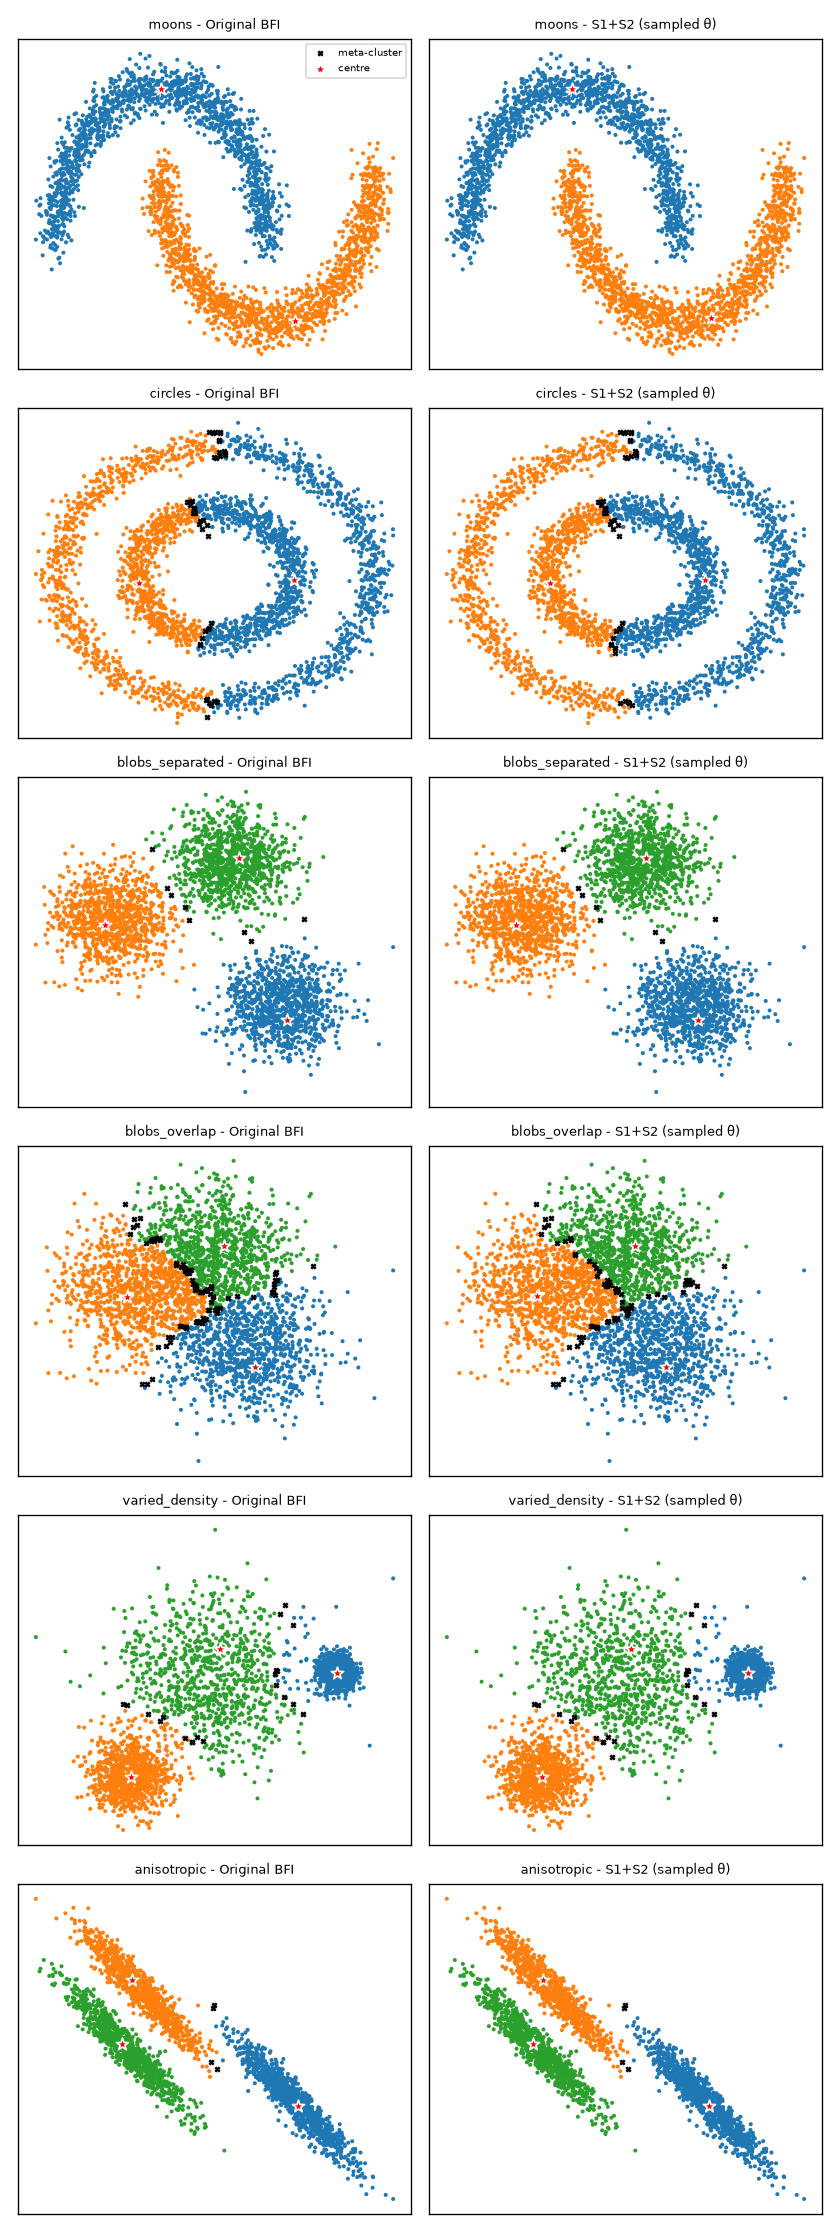
\includegraphics[height=0.78\textheight,keepaspectratio]{exp1_clusters.png}
\caption{Clustering results by the original BFI (left) and S1+S2$^{\dagger}$ (right) on the six 2-D datasets ($N=3000$). Red stars: cluster centres; black crosses: objects assigned to meta-clusters.}
\label{fig:clusters}
\end{figure}

\begin{figure}[!t]
\centering
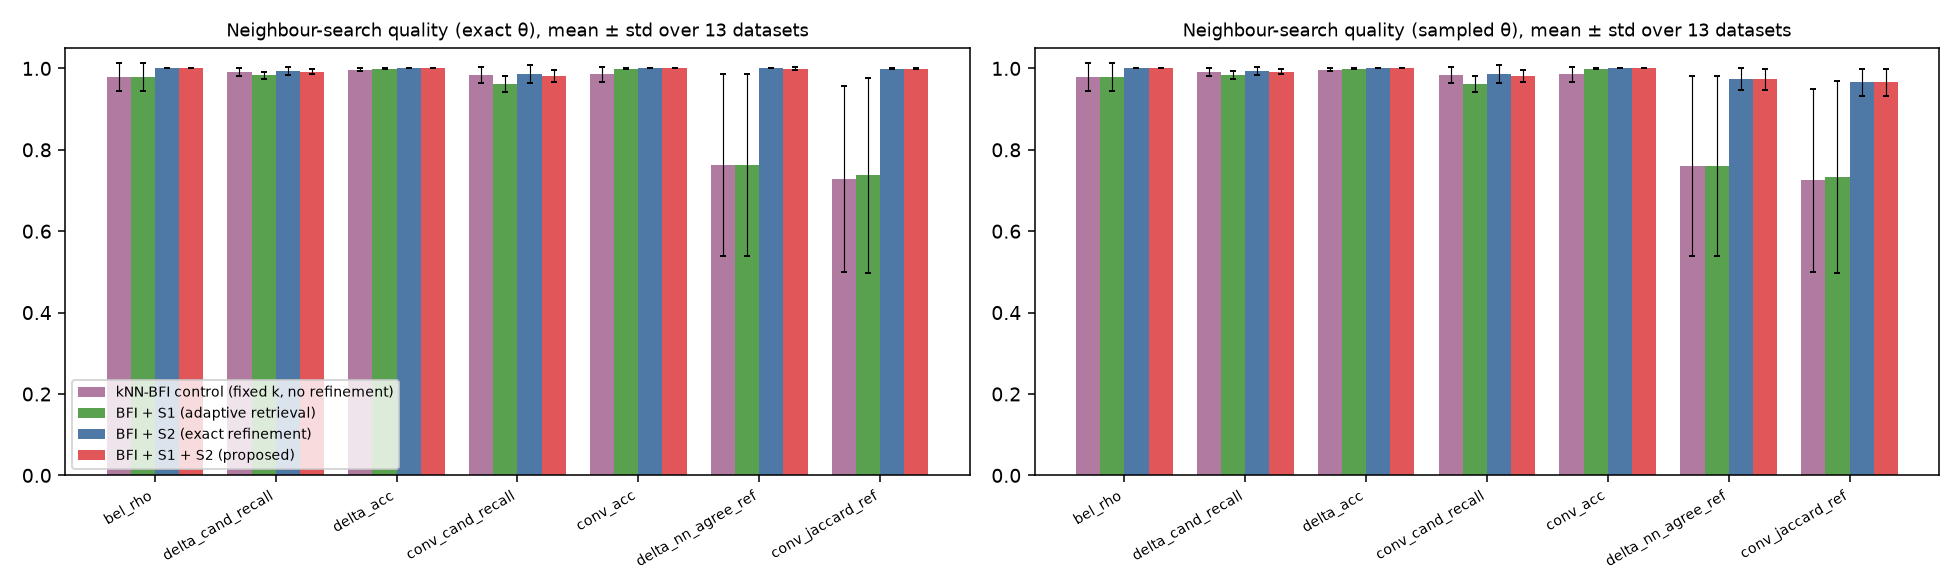
\includegraphics[width=\columnwidth]{exp1_neighbour_accuracy.png}
\caption{Neighbour-search accuracy of the compared methods (exact $\vartheta$, 13 datasets).}
\label{fig:neigh}
\end{figure}

\emph{2) Experiment 2:} This study evaluates the scalability of the methods on the Gaussian mixture with $N=1000$ to 50\,000 (Table~\ref{tab:scal}, Fig.~\ref{fig:scal}). Only 0.47\,GB of RAM was free during this run, so the original BFI was run up to $N=4000$; larger sizes would have swapped and distorted its timing. The memory of the original grows by a factor of 3.7--4.0 per doubling of $N$, i.e., quadratically. The memory of S1+S2 grows only from 12 to 38\,MB over a 50-fold increase of $N$. At $N=4000$, peak memory falls from 366\,MB to 26\,MB ($14\times$), and the runtime from 0.401\,s to 0.173\,s ($2.31\times$). The speed-up grows with $N$. At $N=50\,000$, S1+S2 needs 14.6\,s and 38\,MB, whereas the distance matrix alone would need about 20\,GB. The label agreement with the original remains $\ge0.999$, and ARI stays at 0.917--0.924 for every $N$.

S1+S2 needs about eight exact convergence scans per run at every $N$ from 2000 to 50\,000. Without refinement, the number of estimated queries grows with $N$ (control: 12 to 1951; S1: 3 to 142; Fig.~\ref{fig:work}). As a result, at $N=50\,000$ the ARI falls to 0.265 for the control and 0.396 for S1, whereas S2 and S1+S2 reach 0.924.

\begin{table}[!t]
\centering
\caption{Scalability on the Gaussian mixture (mean of 3 seeds)}
\label{tab:scal}
\scriptsize
\setlength{\tabcolsep}{3pt}
\begin{tabular}{rccccc}
\toprule
$N$ & Original & S1+S2$^{\dagger}$ & Speed-up & Agreement & ARI \\
 & time / memory & time / memory & & & \\
\midrule
1\,000 & 0.037\,s / 25\,MB & 0.031\,s / 12\,MB & 1.18 & 1.000 & 0.917 \\
2\,000 & 0.116\,s / 92\,MB & 0.070\,s / 9\,MB & 1.67 & 0.999 & 0.917 \\
4\,000 & 0.401\,s / 366\,MB & 0.173\,s / 26\,MB & \textbf{2.31} & 0.999 & 0.917 \\
10\,000 & -- & 0.742\,s / 28\,MB & -- & -- & 0.919 \\
20\,000 & -- & 2.53\,s / 30\,MB & -- & -- & 0.923 \\
50\,000 & ($\approx$20\,GB) & 14.6\,s / 38\,MB & -- & -- & 0.924 \\
\bottomrule
\end{tabular}
\end{table}

\begin{figure}[!t]
\centering
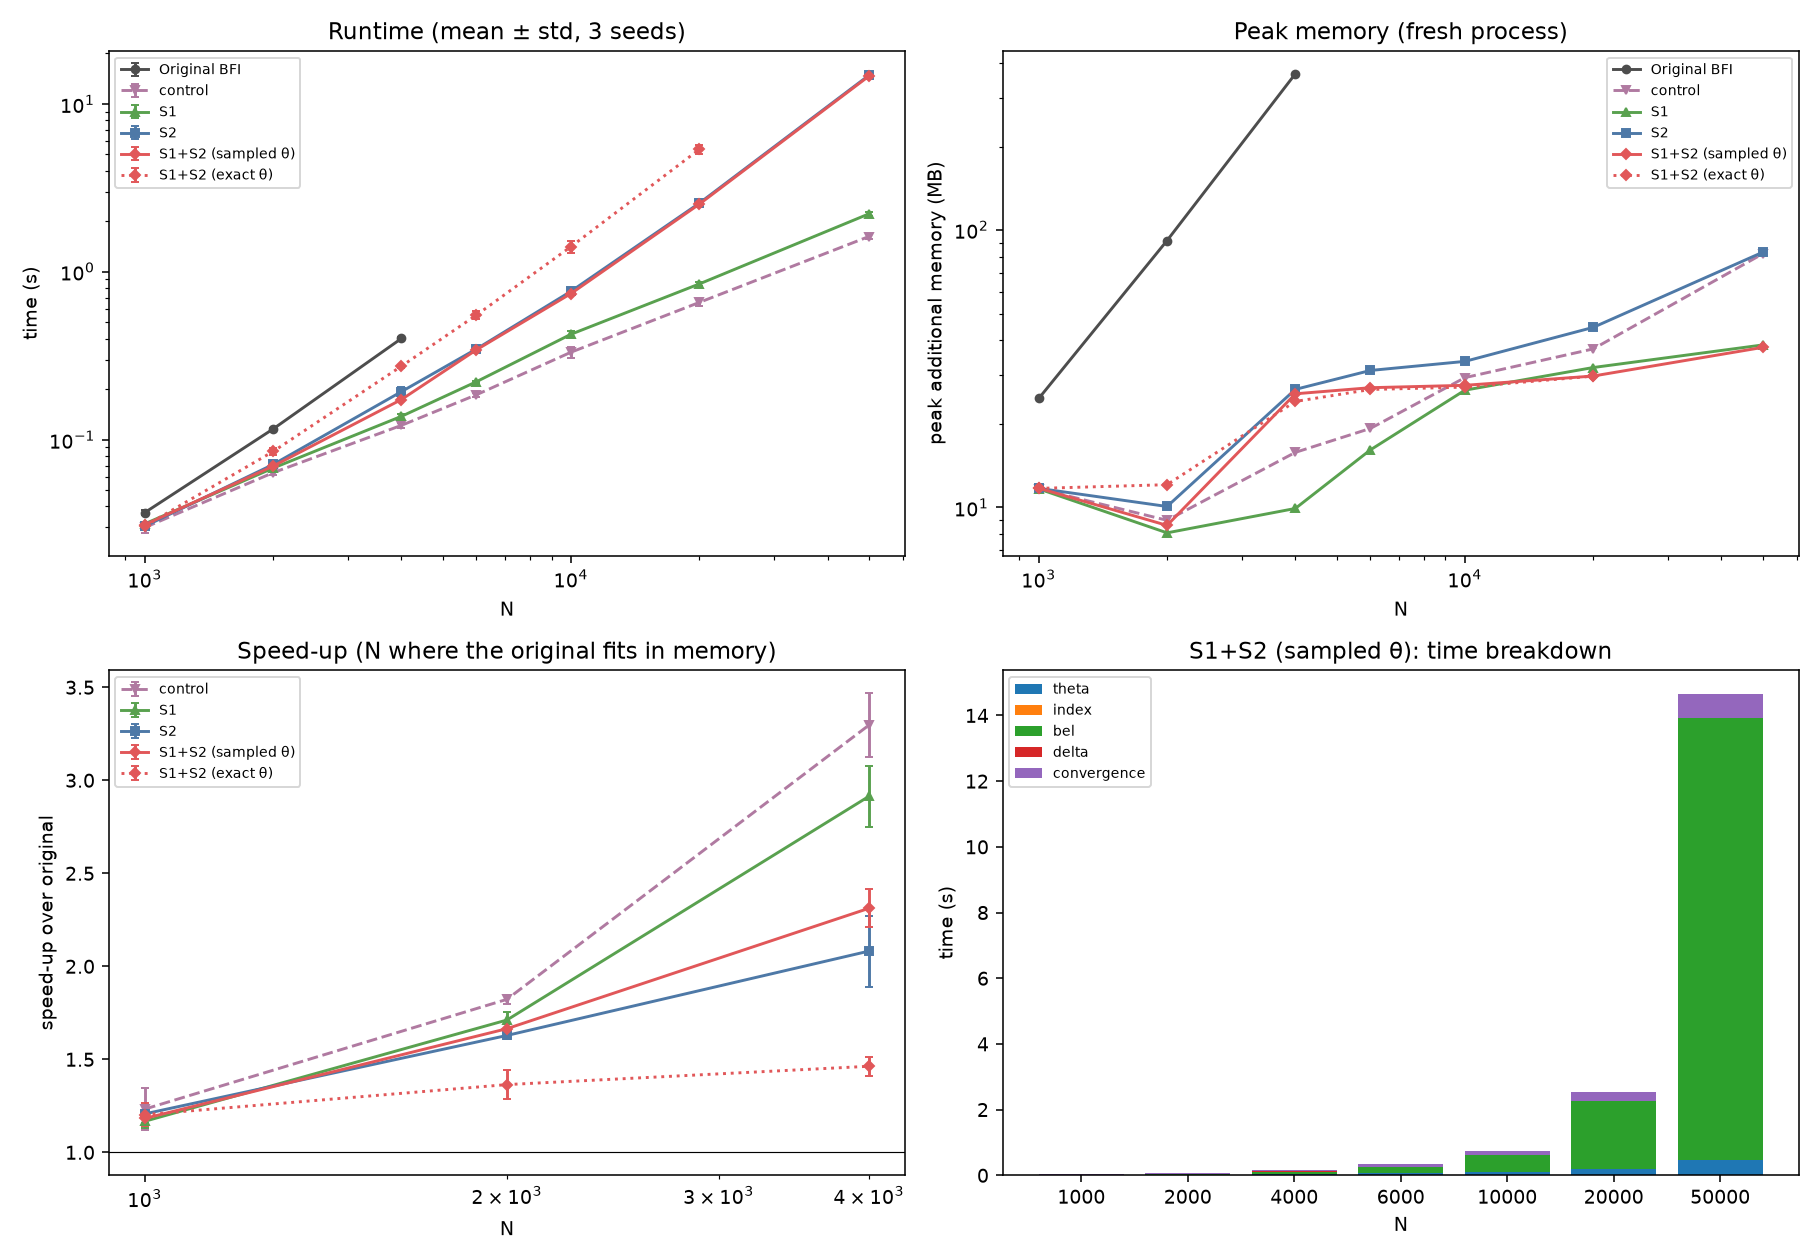
\includegraphics[width=\columnwidth]{exp2_scalability.png}
\caption{Runtime, peak memory, speed-up and time breakdown of S1+S2$^{\dagger}$ versus $N$.}
\label{fig:scal}
\end{figure}

\begin{figure}[!t]
\centering
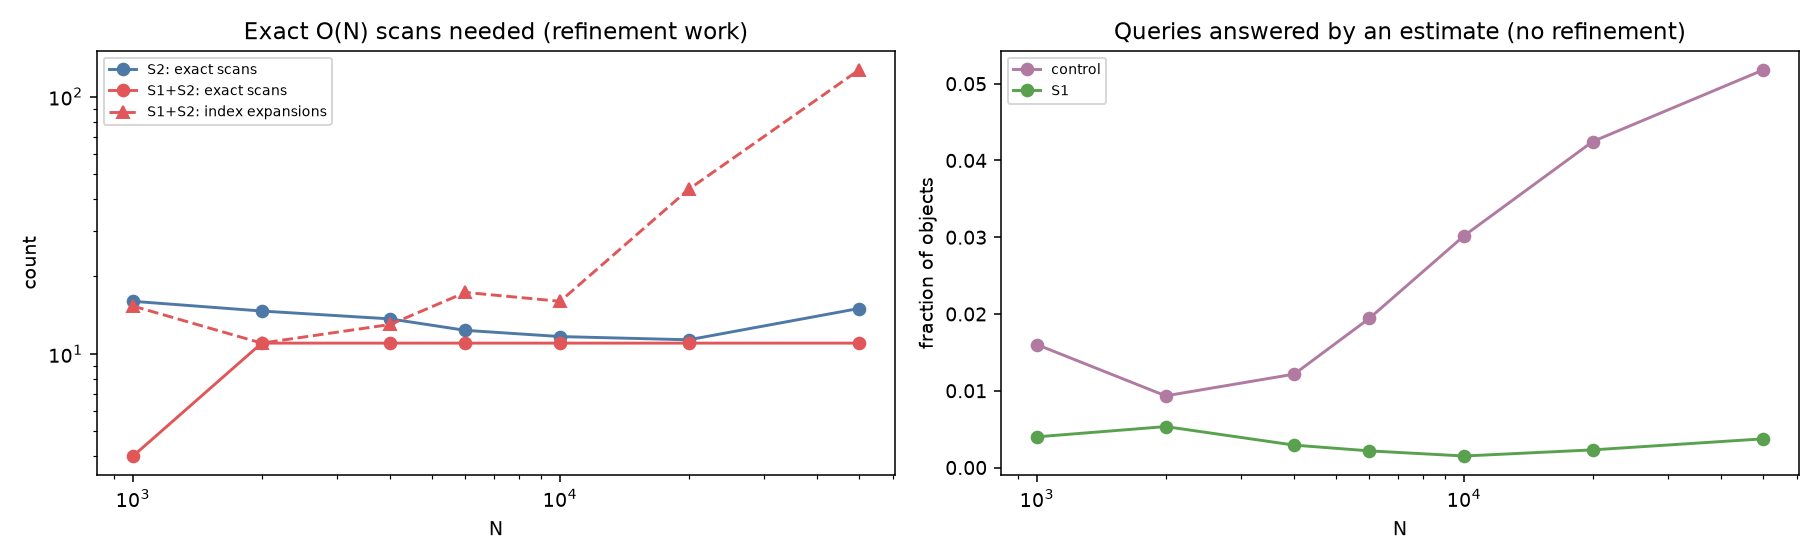
\includegraphics[width=\columnwidth]{exp2_refinement_work.png}
\caption{Exact scans needed by refinement (left) and queries answered by an estimate when refinement is disabled (right).}
\label{fig:work}
\end{figure}

\emph{3) Experiment 3:} This study analyses the contribution of each component on four datasets (varied\_density, blobs\_overlap, moons, blobs\_hd8) at $N=4000$, with three seeds and exact $\vartheta$ (Table~\ref{tab:factorial}, Fig.~\ref{fig:factorial}).
\begin{enumerate}
\item[a)] \emph{Effect of Solution~2:} Refinement provides exactness. The agreement rises from 0.835 (control) or 0.914 (S1) to 1.000, at a cost of about 20\% runtime at this size.
\item[b)] \emph{Effect of Solution~1:} Adaptive retrieval reduces the mean convergence list from 64 to about 18 entries. It gives $4\times$ fewer estimated queries without refinement (56.3 to 13.8) and 38\% fewer exact scans with refinement (12.3 to 7.6), at equal speed within the noise.
\item[c)] \emph{Parameters:}
\begin{itemize}
\item $k_{\min}=4$, 8, 16, 32 and 64 give speed-ups of 1.11, 1.35, 1.43, 1.43 and 1.46, and are always exact; $k_{\min}=16$ was chosen.
\item For $k_{\max}$ from 32 to 1024, the speed of S1+S2 is flat (1.44--1.48), while the number of scans falls from 19.3 to 4.2. For S1 alone, agreement peaks at 0.98 with $k_{\max}=512$.
\item Refining all belief values is the only exact policy. Refining only flagged objects or the centre contenders gives agreement 0.949 and 0.893.
\item $s=1000$ gives agreement 0.997 at a $2.15\times$ speed-up.
\end{itemize}
\end{enumerate}
In summary, \emph{refinement guarantees exactness and adaptive retrieval makes refinement cheap}.

\begin{table}[!t]
\centering
\caption{$2\times2$ factorial ablation (mean over 12 dataset--seed pairs, $N=4000$)}
\label{tab:factorial}
\scriptsize
\setlength{\tabcolsep}{3pt}
\begin{tabular}{lccccc}
\toprule
Methods & Speed-up & Agreement & Conv. & Estimated & Mean conv. \\
 & & & scans & queries & list size \\
\midrule
Control & 1.71$\pm$0.25 & 0.835 & 0 & 56.3 & 64.0 \\
S1 & 1.61$\pm$0.25 & 0.914 & 0 & 13.8 & 20.2 \\
S2 & 1.34$\pm$0.25 & \textbf{1.000} & 12.3 & 0 & 66.5 \\
S1+S2 & 1.37$\pm$0.21 & \textbf{1.000} & \textbf{7.6} & 0 & \textbf{17.9} \\
\bottomrule
\end{tabular}
\end{table}

\begin{figure}[!t]
\centering
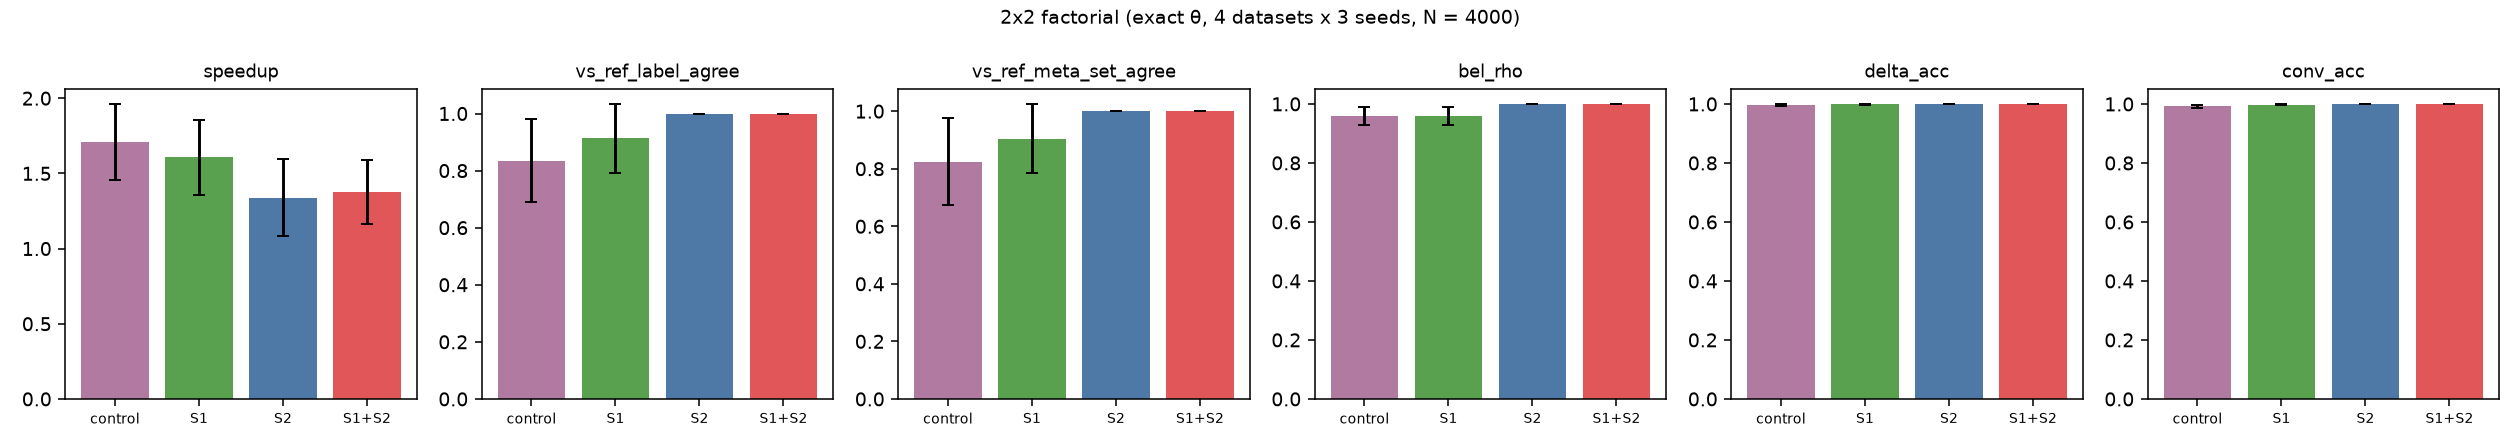
\includegraphics[width=\columnwidth]{exp3_factorial.png}
\caption{Factorial ablation: speed-up, agreement with the original and refinement work of the four configurations.}
\label{fig:factorial}
\end{figure}

\emph{4) Experiment 4:} This study investigates the parameter sensitivity over $K_1\in[0.02N,0.15N]$, $K_2\in\{1,3,5,9,15\}$ and $\zeta\in[0,0.5]$, on four datasets with three seeds and sampled $\vartheta$. S1+S2 follows the original across the whole range. Its agreement is 0.977--0.999 for $K_2\le5$, and 0.90 at $K_2\ge9$, where the original itself collapses (ARI 0.302 and 0.081). The control drops to 45--62\% agreement. As in \cite{zhang2025}, $\zeta$ regulates the number of objects assigned to meta-clusters. The imprecision rate $R_i$ rises from 0 to 0.042 for the original and to 0.040 for S1+S2, while $R_e$ falls from 0.150 to 0.137 and from 0.165 to 0.153, respectively.

\emph{5) Experiment 5:} We also tried to choose the belief candidate count per object from local data, using a two-scale intrinsic-dimension test or an out-of-sample validated power-law tail, so that the $K_1$-neighbour tail could be extrapolated from a short list. At equal mean candidate count, both rules were \emph{worse} than a fixed size (mean relative belief error 0.106 with 66 candidates against 0.054 for a fixed list of 64). The head of a neighbour list carries no information about density changes beyond its radius. Adaptivity is therefore used only where an exact certificate exists, and belief is computed exactly by Solution~2.

%======================================================================
\section{Discussions}\label{sec:disc}
%======================================================================
In this section, we discuss the complexity and the limitations of the proposed method.

\subsection{Complexity Analysis}
Table~\ref{tab:complexity} compares the cost of each step. Building the index costs $O(N\log N)$. The belief pass makes $N$ exact $K_1$-NN queries (expected $O(NK_1\log N)$ in low dimension) with $O(Nk_{\min})$ memory. The $\delta$ and convergence queries cost $O(Nk_{\min})$ for certified objects, plus growth and scans for the few others. In the time breakdown at $N=50\,000$, $\delta$ takes 0.01\,s and the convergence 0.71\,s; both stay cheap at every size.

\begin{table}[!t]
\centering
\caption{Cost of each step (low dimension, expected k-d-tree behaviour)}
\label{tab:complexity}
\scriptsize
\begin{tabular}{lll}
\toprule
Step & Original BFI & Proposed (S1+S2) \\
\midrule
$\vartheta$ & $O(N^2)$ & $O(N^2)$ exact / $O(Ns)$ sampled \\
$\Bel$ & $O(N^2\log N)$ (sort) & $O(NK_1\log N)$ \\
$\delta$ & $O(N^2)$ & $O(Nk_{\min})$ + few scans \\
Convergence & $O(N^2)$ & $O(Nk_{\min})$ + few scans \\
Memory & $O(N^2)$ & $O(Nk_{\min})$ + chunk \\
\bottomrule
\end{tabular}
\end{table}

\subsection{Limitations}
\begin{enumerate}
\item \emph{Exact belief dominates at large $N$:} With $K_1=0.06N$, the belief pass needs $O(N^2)$ distance terms; at $N=50\,000$ it takes 13.5\,s of the 14.6\,s. The quadratic memory and the sort are removed, but not this term.
\item \emph{Exact $\vartheta$ is inherently $O(N^2)$:} At $N\le4000$, the exact-$\vartheta$ configuration is only $1.2$--$1.5\times$ faster than the original. Sampling removes this cost but is the only approximation, and it changes the results on the digits datasets.
\item \emph{High dimension and small datasets:} On blobs\_hd32, the method is slower than the original ($0.61$--$0.75\times$), because k-d trees degrade towards brute force \cite{weber1998}. On real datasets with $N\le1800$, it reaches $0.78$--$1.03\times$. The memory saving remains.
\item \emph{Scope:} The evaluation covers a single machine and a single thread. The Olivetti faces and Berkeley segmentation images of \cite{zhang2025} were not used.
\end{enumerate}

%======================================================================
\section{Conclusion}\label{sec:concl}
%======================================================================
This article introduces an efficient and evidence-preserving framework for belief-based fuzzy and imprecise clustering that changes only how neighbours are retrieved. The adaptive candidate neighbour retrieval answers the $\delta$ and evidential-convergence queries of BFI exactly from short k-d-tree lists, using sufficiency certificates, and enlarges only the lists that need it. The exact distance-based refinement streams exact belief values in bounded memory and resolves the few uncertified queries by restricted exact scans. Experimental findings on 13 datasets and on data with up to 50\,000 objects show three results. First, the method reproduces the original BFI output exactly, including belief values, centres, BBAs and meta-clusters. Second, it reduces memory from quadratic to near-linear (366\,MB to 26\,MB at $N=4000$; 38\,MB at $N=50\,000$). Third, it is up to $2.3\times$ faster. The ablation shows that both components are necessary. The method does not help on high-dimensional or small datasets, and at very large $N$ the exact belief computation dominates the runtime. In the future, we will work on a certified bound on the belief tail, a parallel convergence loop, approximate nearest-neighbour back-ends with recall guarantees for high-dimensional data \cite{malkov2020}, and the image datasets of the original study.

\bibliographystyle{IEEEtran}
\bibliography{references}

\end{document}
